\documentclass[a4paper]{book}
\setcounter{tocdepth}{4}
\setcounter{secnumdepth}{4}
\usepackage{graphicx}
\usepackage{amsmath}
\usepackage{amsfonts}
\usepackage{amssymb}
\usepackage{geometry}
\usepackage{float}
\geometry{a4paper,scale=0.8}
\usepackage{listings}
\lstset{
	basicstyle=\sffamily,
	keywordstyle=\bfseries,
	commentstyle=\rmfamily\itshape,
	stringstyle=\ttfamily}
\begin{document}

\sffamily
\author{Hu Xiping}
\title{Note on Mathematica Programming}
\date{\today}
\maketitle
\tableofcontents
\part{Basics of Wolfram Language}
\chapter{Features of Mathematica}
\section{Evaluating Commands}
On desktop and web, you may press \textbf{Shift}+\textbf{Enter}. On mobile, press the Wolfram icon vbutton
\section{Auto Complete}
Within the Mathematica notebook, you'll see a variety of aids to help you enter the Wolfram Language.
\section{Studying Resources}
You may RTFM(Read The F***ing Manual) or visit Wolfram website to equip essential skills on Wolfram Language. Or you can JFGI(Just F***ing Google It) if your problem can't be solved. Note that you need to use Google instead of Baidu due to study efficiency and you'd better use English to search for help.
\section{Elementary Arithmetic}
\begin{tabular}{|c|c|c|}
\hline 
Command & Expression & Example \\ 
\hline 
Add & + & 2+2 \\ 
\hline
Subtract & - & 2-2 \\ 
\hline
Multiply & * & 2*2 \\ 
\hline
fDivision & / & 2/2 \\ 
\hline
Power & \^{} & 2\^{}2 \\ 
\hline
Brackets & ( and ) & (2+3)/5 \\
\hline
\end{tabular} 
\chapter{First glance at the Functions}

\section{Usage}
Functions names are all started with capital letters. To use a function, attach a "[]" behind the name of function and input parameters separated with "," into the brackets. Tip: insert a single space after the comma to make your code more visualized.

\noindent\emph{\textbf{Example}}\quad \lstinline[language=Mathematica]|Plus[3,4,5]| \hspace{\fill}\emph{Output:} $12$

\noindent You may use the output of function as a parameter of other functions.

\noindent\emph{\textbf{Example}}\quad \lstinline[language=Mathematica]|Times[2,Plus[2,3]]| \hspace{\fill}\emph{Output:} $7$



\subsection{Some basic functions}
\begin{tabbing}
\hspace{0.25\linewidth}\=\hspace{0.25\linewidth}\=\hspace{0.25\linewidth}\=\kill
\lstinline[language=Mathematica]|Plus[2, 3]| \> \lstinline[language=Mathematica]|Subtract[2, 3]| \> \lstinline[language=Mathematica]|Times[2, 3]| \> \lstinline[language=Mathematica]|Divide[2, 3]| \\
\lstinline[language=Mathematica]|Power[2, 3]| \> \lstinline[language=Mathematica]|Max[2, 3]| \> \lstinline[language=Mathematica]|Min[2, 3]| \> \textbf{RandomInteger}[100] \\ 
\end{tabbing} 
\chapter{Introduction to Lists}
\section{List is a way to store numbers}
\emph{\textbf{Example}}\quad
\lstinline[language=Mathematica]|{1,2,3,4,5}| is a list
\section{Create a List}
\subsection{Range[] is a basic function to create lists}

\noindent\emph{\textbf{Example}}\quad \lstinline[language=Mathematica]|Range[10]| \hspace{\fill}\emph{Output:} $\{1,2,3,4,5,6,7,8,9,10\}$

\paragraph{Note}\lstinline[language=Mathematica]|Range[m,n,p]| means a list start with m, end with n, in step of p

\noindent\emph{\textbf{Example}}\quad \lstinline[language=Mathematica]|Range[3,7]| \hspace{\fill}\emph{Output:} $\{3,4,5,6,7\}$

\noindent\emph{\textbf{Example}}\quad \lstinline[language=Mathematica]|Range[2,10,3]| \hspace{\fill}\emph{Output:} $\{2,5,8\}$

\subsection{IntegerDigits[] convert number to list}
\noindent Use \textbf{IntegerDigits} to create lists out of integer number
\newline
\noindent\emph{\textbf{Example}}\quad \lstinline[language=Mathematica]|IntegerDigits[1988]| \hspace{\fill}\emph{Output:} \lstinline[language=Mathematica]|{1,9,8,8}|

\subsection{Use Table to create List iteratingly}
\label{subsec:label}

\subsubsection{Repeated}
\emph{Usage:} \lstinline[language=Mathematica]|Table[content,times]| 
\newline
\noindent\emph{\textbf{Example}}\quad \lstinline[language=Mathematica]|Table[2,5]| \hspace{\fill}\emph{Output:} \lstinline[language=Mathematica]|{2,2,2,2,2}|
\newline
\noindent\emph{\textbf{Example}}\quad \lstinline[language=Mathematica]|Table[x,4]| \hspace{\fill}\emph{Output:} \lstinline[language=Mathematica]|{x,x,x,x}|
\newline
\noindent\emph{\textbf{Example}}\quad \lstinline[language=Mathematica]|Table[{1,2},3]| \hspace{\fill}\emph{Output:} \lstinline[language=Mathematica]|{{1,2},{1,2},{1,2}]}|
\newline
\subsubsection{Iterating}
\noindent Iterate from 1 to n
\newline
\emph{Usage:} \lstinline[language=Mathematica]|Table[expression, {varibale,n}]|
\newline
\noindent\emph{\textbf{Example}}\quad \lstinline[language=Mathematica]|Table[x^2,{x,4}]| \hspace{\fill}\emph{Output:} \lstinline[language=Mathematica]|{1,4,9,16}|
\newline
\noindent\emph{\textbf{Example}}\quad \lstinline[language=Mathematica]|Table[Range[expt],{expt,3}]| \hspace{\fill}\emph{Output:} \lstinline[language=Mathematica]|{{1},{1,2},{1,2,3}}|
\newline
\newline
\noindent Iterate from m to n
\newline
\emph{Usage:} \lstinline[language=Mathematica]|Table[expression, {varible,m,n}]|
\newline
\noindent\emph{\textbf{Example}}\quad \lstinline[language=Mathematica]|Table[f[n],{n,4,7}]| \hspace{\fill}\emph{Output:} \lstinline[language=Mathematica]|{f[4],f[5],f[6],f[7]}|
\newline
\newline
\noindent Iterate from m to n in steps of p
\newline
\emph{Usage:} \lstinline[language=Mathematica]|Table[expression, {m,n,p}]|
\newline
\noindent\emph{\textbf{Example}}\quad \lstinline[language=Mathematica]|Table[g[a],{4,10,2}]| \hspace{\fill}\emph{Output:} \lstinline[language=Mathematica]|{g[4],g[6],g[8],g[10]}|
\newline
\newline
\noindent Use 2 variables to iterate
\newline
\noindent\emph{\textbf{Example}}\quad \lstinline[language=Mathematica]|Table[i, {i, 4}, {j, 5}]| \newline
\phantom{x}\hspace{\fill}\emph{Output:} \lstinline[language=Mathematica]|{{1, 1, 1, 1, 1}, {2, 2, 2, 2, 2}, {3, 3, 3, 3, 3}, {4, 4, 4, 4, 4}}|
\newline






\section{Visualizing Lists}

\subsection{ListPlot}

\emph{\textbf{Example}}\quad\lstinline[language=Mathematica]|ListPlot[1,2,3,4,3,4]|
\begin{figure}[H]
  \centering
  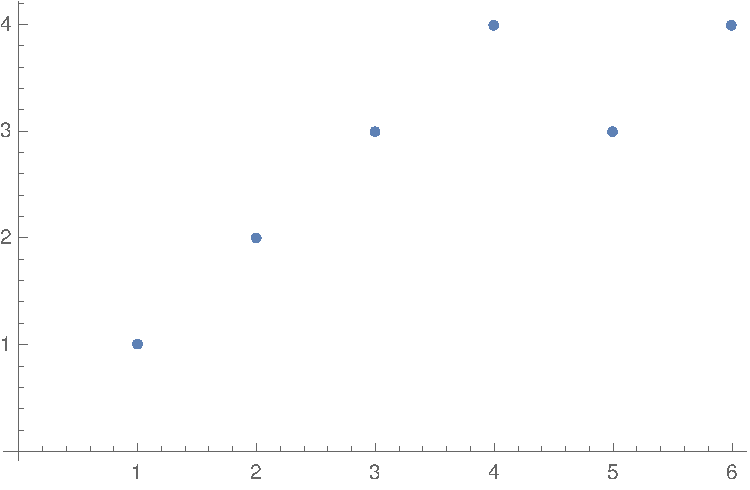
\includegraphics[width=0.45\linewidth]{figures/ListPlot}
  \caption{ListPlot}
\end{figure}



\noindent\emph{\textbf{Example}}\quad\lstinline[language=Mathematica]|ListPlot[Join[Range[20]], Reverse[Range[20]], Range[30]]|

\begin{figure}[H]
  \centering
  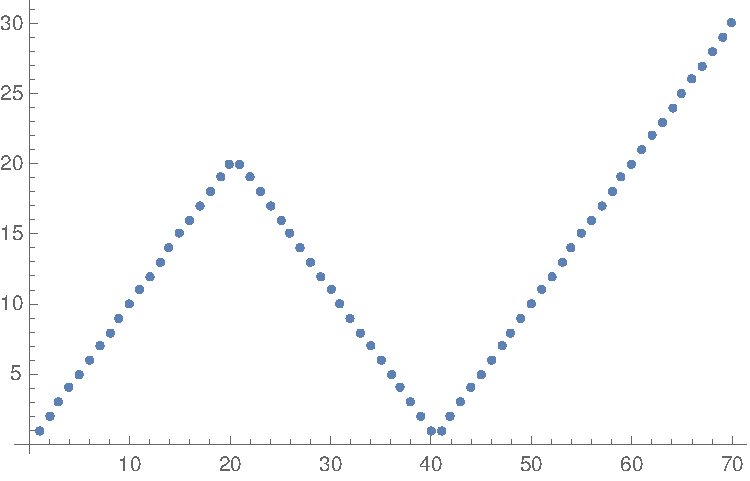
\includegraphics[width=0.45\linewidth]{figures/ListPlot2}
  \caption{ListPlot}
\end{figure}


\subsection{ListLinePlot}
\label{subsec:label}
\noindent\emph{\textbf{Example}}\quad\textbf{ListLinePlot}\lstinline[language=Mathematica]|[{1.5, 2, 4, 2.3, -9}]|
\begin{figure}[H]
  \centering
  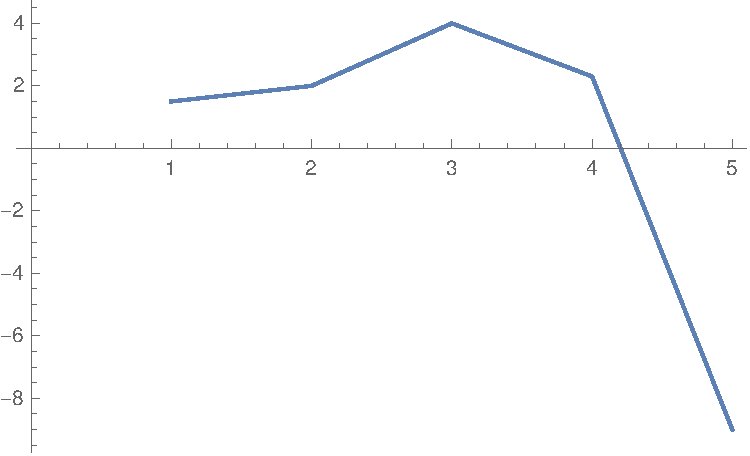
\includegraphics[width=0.45\linewidth]{figures/ListLinePlot.pdf}
  \caption{ListLinePlot}
\end{figure}

\subsection{BarChart}
\label{subsec:label}

\noindent\emph{\textbf{Example}}\quad\textbf{BarChart}\lstinline[language=Mathematica]|[{1.5, 2, 4, 2.3, -9}]|



\begin{figure}[H]
  \centering
  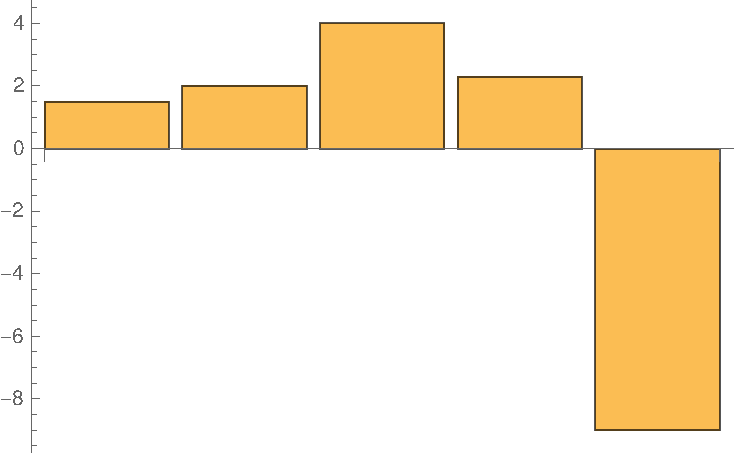
\includegraphics[width=0.45\linewidth]{figures/BarChart}
  \caption{BarChart}
\end{figure}

\subsection{PieChart}
\label{subsec:label}

\noindent\emph{\textbf{Example}}\quad
\textbf{BarChart}\lstinline[language=Mathematica]|[{1, 3, 5, 4}]|
\begin{figure}[H]
\begin{minipage}{.5\linewidth}
  \centering
  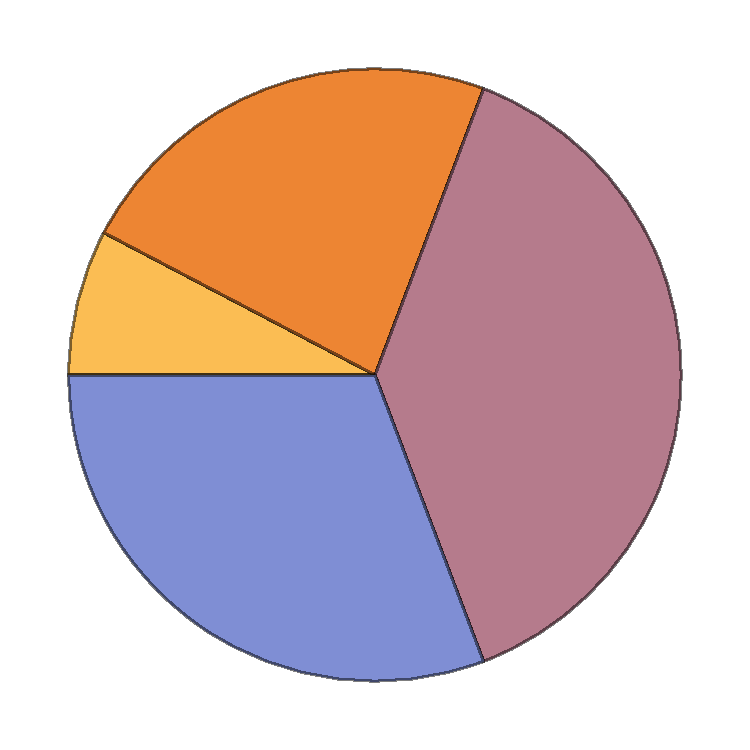
\includegraphics[width=0.7\linewidth]{figures/PieChart}
  \caption{PieChart}
\end{minipage}\begin{minipage}{.5\linewidth}
  \centering
  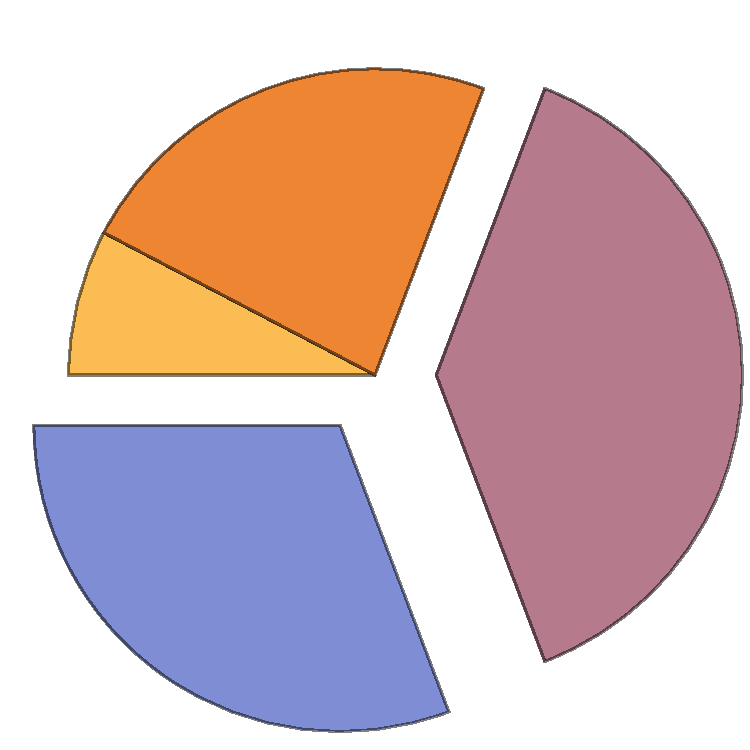
\includegraphics[width=0.7\linewidth]{figures/PieChart2}
  \caption{Interact with PieChart segments}
\end{minipage}
\end{figure}

\noindent\emph{Note that You can also left click on the chart to interact with the segments}

\subsection{NumberLinePlot}
\label{subsec:label}

\emph{\textbf{Example}}\quad\textbf{NumberLinePlot}\lstinline[language=Mathematica]|[{2, 3, 1, 5, -6.2}]|

\begin{figure}[H]
  \centering
  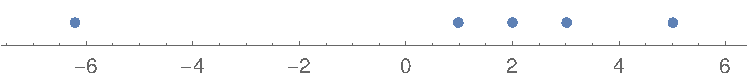
\includegraphics[width=0.45\linewidth]{figures/NumberLinePlot}
  \caption{NumberLinePlot}
\end{figure}






\section{Advanced Operation on List}
\label{sec:label}

\subsection{Operate with Basic arithmetic operators}
\label{subsec:label}

\subsubsection{Operate with numbers}
\noindent\emph{\textbf{Example}}\quad\lstinline[language=Mathematica]|{1, 2, 3} + 10|\hspace{\fill}\emph{Output:} \lstinline[language=Mathematica]|{11,12,13}|

\noindent\emph{\textbf{Example}}\quad
\lstinline[language=Mathematica]|{1,2,3}-10|\hspace{\fill}\emph{Output:} \lstinline[language=Mathematica]|{-9,-8,-7}|


\noindent\emph{\textbf{Example}}\quad
\lstinline[language=Mathematica]|{1,2,3}*10}|\hspace{\fill}\emph{Output:} \lstinline[language=Mathematica]|{10,20,30}|

\noindent\emph{\textbf{Example}}\quad\lstinline[language=Mathematica]|{1,2,3}/10|\hspace{\fill}\emph{Output:} \{$\frac{1}{10},\frac{1}{5},\frac{3}{10}$\}

\subsubsection{Operate with other lists}
\noindent\emph{\textbf{Example}}\quad \lstinline[language=Mathematica]|{1,2,3}+{1,2,3}| \hspace{\fill}\emph{Output:} \{2,3,4\}

\noindent\emph{\textbf{Example}}\quad \lstinline[language=Mathematica]|{1,2,3}-{2,3,4}| \hspace{\fill}\emph{Output:} \{-1,-1,-1\}

\noindent\emph{\textbf{Example}}\quad \lstinline[language=Mathematica]|{1,2,3}*{1,2,3}| \hspace{\fill}\emph{Output:} \{1,4,9\}

\noindent\emph{\textbf{Example}}\quad \lstinline[language=Mathematica]|{1,2,3}/{2,3,4}| \hspace{\fill}\emph{Output:} \{$\frac{1}{2},\frac{2}{3},\frac{3}{4}$\}

\subsection{Operate with Functions}

\subsubsection{Whole list operation}

\noindent Join lists together
\newline
\noindent\emph{\textbf{Example}}\quad \lstinline[language=Mathematica]|Join[Range[3],Range[5],Range[3]]| \hspace{\fill}\emph{Output:} $\{1,2,3,1,2,3,4,5,1,2,3\}$
\newline
\newline
\noindent Reverse elements
\newline
\noindent\emph{\textbf{Example}}\quad \lstinline[language=Mathematica]|Reverse[\{1,2,3\}]| \hspace{\fill}\emph{Output:} $\{3,2,1\}$
\newline
\newline
\noindent Length of the list
\newline
\noindent\emph{\textbf{Example}}\quad \lstinline[language=Mathematica]|Length[{5,3,4,2,3,4}]| \hspace{\fill}\emph{Output:} $6$
\newline
\newline
\noindent Sum up
\newline
\noindent\emph{\textbf{Example}}\quad \lstinline[language=Mathematica]|Total[{1,2,3}]| \hspace{\fill}\emph{Output:} $6$
\newline
\newline
\noindent Sort the elements
\newline
\noindent\emph{\textbf{Example}}\quad \lstinline[language=Mathematica]|Sort[{6,7,1}]| \hspace{\fill}\emph{Output:} \lstinline[language=Mathematica]|{1,6,7}| 

\subsubsection{Elements operation}
\noindent See how many times an element appears

\noindent\emph{\textbf{Example}}\quad \lstinline[language=Mathematica]|Count[{a,b,a,a,c,b,a},a]| \hspace{\fill}\emph{Output:} $4$
\newline
\newline
\noindent Extract elements
\newline
\noindent \emph{Usage:} \lstinline[language=Mathematica]|Part[list,position]| 
\newline
\noindent\emph{\textbf{Example}}\quad \lstinline[language=Mathematica]|Part[{7,6,5},2]| \hspace{\fill}\emph{Output:} $6$
\newline
\newline
\noindent Extract the first Element
\newline
\noindent\emph{\textbf{Example}}\quad \lstinline[language=Mathematica]|First[{7,6,5}] (*The same as Part[list,1]*)| \hspace{\fill}\emph{Output:} $7$
\newline
\newline
\noindent Extract the last element
\newline
\noindent\emph{\textbf{Example}}\quad \lstinline[language=Mathematica]|Last[{7,6,5}]| \hspace{\fill}\emph{Output:} $5$
\newline
\newline
\noindent Extract the Max and the Min
\newline
\noindent\emph{\textbf{Example}}\quad \lstinline[language=Mathematica]|Min[{6,7,1}]| \hspace{\fill}\emph{Output:} $1$
\newline
\noindent\emph{\textbf{Example}}\quad \lstinline[language=Mathematica]|Max[{6,7,1}]| \hspace{\fill}\emph{Output:} $7$
\newline
\newline
\noindent Slice the list
\newline
\noindent \emph{Usage:} \lstinline[language=Mathematica]|Take/Drop[list,position]| 
\newline
\noindent\emph{\textbf{Example}}\quad \lstinline[language=Mathematica]|Take[{101,203,401,602,332,412},3]| \hspace{\fill}\emph{Output:} \lstinline[language=Mathematica]|{101,203,401}|
\newline
\noindent\emph{\textbf{Example}}\quad \lstinline[language=Mathematica]|Drop[{102,203,401,602,332,412},3]| \hspace{\fill}\emph{Output:} \lstinline[language=Mathematica]|{602,332,412}| 

\end{document}
